\documentclass[a4paper,12pt,oneside]{book}
%\usepackage{geometry}
%\usepackage{fancyhdr}
%\usepackage{amsmath,amsthm,amssymb }
\usepackage{graphicx}
%\usepackage{lipsum}
\usepackage[utf8]{inputenc}
%\usepackage{ngerman}
%\usepackage{parskip}
\usepackage{textcomp}
\usepackage{float}
\usepackage{hyperref}
\usepackage{placeins}

\setlength{\parskip}{0.2cm}

\hypersetup{
    pdfborder = {0 0 0},		
}

% Hurenkinder und Schusterjungen verhindern
\clubpenalty10000
\widowpenalty10000
\displaywidowpenalty=10000

\pagestyle{plain}

\title{Zeos Documentation Collection}
\author{Jan Baumgarten}
\date{\today}
%\overfullrule=2mm
\begin{document}
\maketitle
\tableofcontents

\chapter{Introduction}
This document is an effort to combine all the available Zeos documentation in one Manual.
It includes a tutorial as found on the Internet and several other pieces.
It is started in the hopes that it somehow will evolve into a kinda manual.

\part{A ZEOS basics tutorial not only for Firebird ...}
This tutorial was originally written by Michael Seeger.

\chapter{Preface}
The ZeosLib DBOs 6.1.5 - With Delphi 7 and Firebird 1.5.
This little article shows how to access Firebird databases by using the ZEOS component Library in version 6.1.5 (including Patches 1\&2) and how to use these components in database applications.
It does not matter if you use the "real" SQL-Server or the embedded version which is restricted to local held databases.
A couple of examples (also migrated Delphi-BDE demos) shall explain how to use the ZEOS
components.

Although this article describes the usage of the ZEOS Library using Firebird, all the basics can be used with other SQL servers / databases that are supported by ZEOS.

Note: The Firebird Server can be downloaded from download section of
http://www.ibphoenix.com
http://www.firebirdsql.org

\chapter{The ZEOS Library}
The name "ZEOS" has no special meaning. The founders of ZEOS found that this name just sounded good.
Since that time the Library is called "ZEOS".

Generally we can say about the ZEOS Library that the developers are inteneded to
copy the functions and the behaviour of the corresponding BDE components as good
as possible.
The intention is to minimize the learning courve for developers who
migrate from BDE to ZEOS.
Of course there must have been made some compromises so that they are not a hundred percent compatible because the ZEOS components shall be applicable universally.

The ZEOS Library in version 6.1.5 consists of the following nine components
which shall be introduced in the following:
\begin{itemize}
\item TZConnection
\item TZQuery
\item TZReadOnlyQuery
\item TZUpdateSQL
\item TZTable
\item TZStoredProc
\item TZSQLProcessor
\item TZSQLMonitor
\item TZSQLMetadata
\end{itemize}

\chapter{Installing the ZEOS Library and additional stuff}

The installation of the ZEOS Library under Delphi 7 professional is not that complicated.
Once the current ZEOS version and all the patches (while writing this article it was library version 6.1.5 and the corresponding patches 1\&2) are downloaded and unzipped into a directory of your choice completely you only have to follow the installation instructions (note: Firebird does not need any additional DLL's, here!):

Open the delphi project group ZeosDbo.bpg from subdirectory packages\textbackslash delphi7 ZeosDbo.bpg and install
the following components in given order:
\begin{itemize}
\item ZCore.bpl
\item ZParseSql.bpl
\item ZPlain.bpl
\item ZDbc.bpl
\item ZComponent.bpl
\end{itemize}

Note: If there occur some errors while compiling that say that a certain dcu file could not be found then just add the subdirectory packages\textbackslash delphi7\textbackslash build to delphis library path.
All dcu files that are created while compilation are located here.

Attention: The client library of Firebird Server version 1.5.1 (not embedded!) was delivered as "gds32.dll" and not "fbclient.dll".
This causes trouble while accessing via ZEOS because the protocol "firebird1.5" assumes a DLL named "fbclient.dll".
A workaround is to copy the "gds32.dll" and rename this copy to "fbclient.dll".

\chapter{Basics: Transactions}
Some mandatory basics about transactions have to be told in order to understand how the TZConnection
component works internally and how to work with it.

In general: You only can have access to a database within the context of a valid ("running") transaction.
A transaction has to fulfill the following four characteristics that are known as ACID characteristics of a transaction.

Atomicity: All actions performed on a database have to be executed successfully.
If only one error occurs then the original state of the database has to be restored.
According to the principle "all or nothing".

Consitency: A transaction transfers a database from one consitent state to an other consistent state.
If an error occurs then the original state of the database has to be restored.

Isolation: A transaction has to be handled by the server as if it was the only one running.
This means it has to run indepently from other transactions.
A user must not notice the changes done by other users.

Durability: Changes in the dataset of a database that are caused by SQL statements that are executed between the start of a transaction and a COMMIT have to be fixed irrevocably.

Transactions encapsulate consecutive accesses on a database.
A database access may be of reading or writing nature (INSERT, UPDATE, DELETE) or it may change the structure of a database.
Transactions are terminated by COMMIT or ROLLBACK.
COMMIT confirms all changes in a database since the start of a transaction.
ROLLBACK resets all changes in a database since the start of a transaction.

Transactions running on the server have to be isolated from each other.
So they may run independently.
A transaction has to be handled by the server as it was the only one that is currently running.
This means for the user that he must never see the changes of other users while he is in a running transaction because the other changes have nothing to do with his transaction.
This is called the isolation of a transaction.
By using different transaction isolation levels (TILs) the developer may protect the data of an SQL resultset from access by other transactions.
The behaviour described above is called the standard isolationlevel known as SERIALIZABLE.
The standard isolationlevel of Firebird is called SNAPSHOT and comes very close to SERIALIZABLE.

\chapter{The Zeos Components}

\section{TZConnection}
The TZConnection component is a combination of a BDE TDatabase like component a component that
handles a transaction.
This combination makes sense because all access to a Firebird database (and also other databases) is always made in a running transaction.
Such a transaction is startet by the ZEOS Library whenever a connection (method Connect of TZConnection) to a database is opened.
This causes that each database access is done within the context of a running transaction, automatically.
The so called AutoCommit mode is always on (set to "True").
This is also the standard behaviour of the corresponding BDE component.
If AutoCommit is activated then every change of an SQL statement will be confirmed in the
database by COMMIT ater its successfull execution.
If this behaviour shall be turned off and an explicit transaction shall be started then the method StartTransaction has to be called.
Within this explicit transaction it is possible to execute a couple of SQL statements that make changes to the database, in succession.
These statements then can be confirmed as a "group" by COMMIT.
If an explicit transaction is active then AutoCommit is always turned off.
By Calling the Method Commit all the changes made within this explicit transaction are confirmed.
Calling the method Rollback resets these changes.
In both cases AutoCommit will be set to True when the method call (Commit or Rollback) is done.
The explicit transaction has ended.

\subsection{Retaining}
After confirming the chanes made in a transaction by COMMIT or resetting them by ROLLLBACK the
transaction normally is going to be ended and an existing resultset of a query or stored procedure will be discarded.
These COMMITs and ROLLBACKs are called "hard" commit or "hard" rollback.
By using the ZEOS library this will become a little bit different.
ZEOS keeps the resultset alive.
This is achieved by closing transaction with "soft" commits or "soft" rollbacks.
All this is done by the TZConnection object.
This method is called retaining.
The COMMIT and ROLLBACK commands are executed with the addition RETAINING.
Retaining causes the closing of the current transaction and immediately opening a new transaction with all the data and resources (especially the resultset) of the "old" transaction.

Retaining becomes a problem if it is uses for huge tables.
It constrains the internal cleanup mechanism of firebird (garbage collection).
This leads (because of the versioning and the multigenerational architecture of Firebird) to a lot of old records that have to be kept but will not be needed anymore.
This influences the server's performanced in a negative way.
A so called sweep would discard these old versions and improve the performance.
This sweep will only be executed by sending a "hard" COMMIT or ROLLBACK.
The ZEOS Library only executes these "hard" commands when ending the database connection (closing connection).
It is not possible to send them while a database connection is active. So the database connection should be deactivated and immediately activated occasionally to achieve this performance improvement.

\subsection{Transaction Isolation Levels of TZConnection}

The TZConnection component provides four useful and predefined Transaction Isolation Levels (TIL):

tiRepeatableRead:
It corresponds to the TIL "SNAPSHOT" which is the standard of Firebird servers.
It is a combination of the trasaction parameters "concurrency" and "nowait".
A snapshot of the current database is made.
Other users are only influenced (constrained) if two transactions work on one record simultaneously.
If conflicts arise while accessing data an error message will be returned.
Changes within other transactions will not be noticed.
This TIL covers the requirement of the SQL standard (SERIALIZABLE) widely.

tiReadCommitted:
It corresponds to the TIL "READ COMMITTED".
It is a combination of the transaction parameters "read\_committed", "rec\_version" and "nowait".
This TIL recognizes all changes in other transaction that have been confirmed by COMMIT.
The parameter "rec\_version" is responsible for the behaviour that the most current values that were committed by other users will be considered.
The parameter "nowait" is resposible for the behaviour that there is no waiting for the release of a locked record.
So the server is more stressed than in TIL tiRepeatableRead because it has to do all the refreshes to get these values again and again.

tiSerializable:
It corresponds to the TIL "SNAPSHOT TABLE STABILITY".
It is used to get an exclusive access to the result set.
Realized by transaction parameter "consistency" it prevents that "foreign" transaction may access the written data.
Only the transaction which has written the data may access them.
This prevents also a multi user access to the written data.
Because this TIL is very restrictive by accessing written data it should be applied with caution and care.

tiNone: No TIL is used to isolate the transaction.

The TIL tiReadUncommitted is not supported by Firebird.
If this TIL is used, an error will be triggerded and the transaction will not be isolated (like using tiNone).

\subsection{Recommendation}
It is advisable to isolate transactions with transaction isolation level tiRepeatableRead (the Firebird standard).
This TIL covers the requirement of the SQL standard (SERIALIZABLE) widely.
It prevents all problems concerning consistency that may arise by using transactions.
Second choice would be tiReadCommitted but this depends on the application and the necessity if the reseult set always has to be current.

\subsection{Customizing TILs}

If you want to customize your TILs or expand a given TIL then you can do this by using the parameters of TZConnection.
The most important thing about this is that the TIL that should be expanded has to be set in
property IsolationLevel.
If it is set the TIL parameters (see IB/FB API reference) you want to add may be added in sourcecode.
The following example shows the expansion of a TIL preset to tiNone:
\begin{verbatim}
ZConnection.TransactIsolationLevel := tiNone;
ZConnection.Properties.Add('isc\_tpb\_concurrency');
ZConnection.Properties.Add('isc\_tpb\_wait');
ZConnection.Connect;
\end{verbatim}

\subsection{Protocol}
The most important setting in a TZConnection object is the server protocol it is set in property Protocol.
It determines which protocol shall be used and thus which SQL server will be accessed.
This method makes ZEOS so flexible.
You don't have to install special components for each database you want to access as it was in Versions 5.x and earlier.
The components will be installed once.
This is enough.
You only choose the protocol for the supported SQL server you want to access and you are done.
So you set protocol "firebird1.5" to access Firebird 1.5 server.

\subsection{Read-Only-Connection}

The database connection maintained by a TZConnection object is set to read only by default (ReadOnly = True).
This means that no writing access to the connected database is allowed.
To get writing access to the database you have to set ReadOnly to False.

\subsection{Codepages}
Codepages will be determined by setting parameter "lc\_ctype" or "Codepage" in TZConnection.
This parameter must be added to the property Properties. E. g.:
\begin{verbatim}
ZConection.Properties.Add ('lc\_ctype=ISO8859\_1');
\end{verbatim}
or
\begin{verbatim}
ZConnection.Properties.Add ('Codepage=ISO8859\_1');
\end{verbatim}

Note: The Codepage support of Firebird (also embedded version) in version 1.5 with ZEOS is a little bit buggy. These bugs are corrected in Firebird version 1.5.1.

\subsection{Features of the Firebird embedded server}

Normally the server name or IP address of the server is given in property HostName.
By using a Firebird embedded server you may leave this property empty.
Only property Database has to be determined.
Here you have to specify drive path and name of the database including extension.

An other feature of the embedded server is that you may specify any login name with a pasword of your choice.
It doesn't matter what you choose you will get connected.

Setting the TZConnection object property Connected to True in designtime is extremely bad if you don't reset it to False before compiling.
If you then start the compiled application with IDE running you will get an error that says that the database cannot be opened because it is already in use.
So you should establish the connection to the database when starting the application (e. g. in OnCreate event of the main form) and then open the needed queries and tables.
Deactivating the connection should also be done in main form (e. g. in OnDestroy).
It is not necessary to close all open queries and tables.
This will be done when closing the connection of the TZConnection object.
If you use datamodel forms you have to take care that the datamodel form is created before the main form is created (set in the IDE's project options)...

\subsection{Useful TZConnection parameters}

Additional parameters for establishing connections to Firebird databases are:

CreateNewDataBase:
A new database will be created based on the specified CREATE DATABASE statements.
When the database is created the connection will be established immediately.
All this happens by calling the Connect method of TZConnection.
\begin{verbatim}
ZConnection1.Database := 'd:\db1.fdb';
ZConnection1.Protocol := 'firebird-1.5';
ZConnection1.Properties.Add ('CreateNewDatabase=CREATE DATABASE ' + QuotedStr ('d:\db1.fdb') + ' USER ' + QuotedStr ('sysdba') + ' PASSWORD ' + QuotedStr ('masterkey') + ' PAGE\_SIZE 4096 DEFAULT CHARACTER SET ISO8859\_1');
ZConnection1.Connect;
\end{verbatim}

To execute this correctly you have to set the Database and Protocol properties at minimum (also possible in objectinspector).

Dialect:
This parameter sets Firebird's SQL dialiect. To set dialect "1" you have to use the following code:
\begin{verbatim}
ZConnection.Properties.Add ('Dialect=1');
\end{verbatim}

The dialect of Firebird 1.5.x is set to "3" by default.

Rolename:
This parameter sets a rolename. A logged in user then works in the context of the role's rights but before the user has to be assigned to this role.
The Firebird embedded server does not support this feature.

\section{TZQuery}

The usage of TZQuery is similar to the usage of BDE's TQuery component.

\subsection{Recommandation: RequestLive and TZUpdateSQL}
If an SQL dataset shall be updatable then RequestLive has to be set to true and you should generally use according update SQL statements that will be defined in TZUpdateSQL.
If this is done just assign TZUpdateSQL to the TZQuery object.
Now all changes that will be made in the result set will be done to the database by using the defined statements of TZUpdateSQL.
According to experience RequestLive mode runs more smoothly by using TZUpdateSQL.

\subsection{Usage of parameters in SQL statements}

Using parameters in SELECT statments is as easy as using them with BDE's TQuery.
If TZQuery has a result set then you have to use the Open method.
If you want to execute an SQL statement which has no result set (e. g.: INSERT or UPDATE) you have to use ExecSQL (see also: TZStoredProc).

\section{TZReadOnlyQuery}

This is a Query component that is quite similar to the TZQuery component.
There is just one difference:
The result set is read only.
There is no possibility to assign a TZUpdateSQL object.

\section{TZUpdateSQL}

A TZUpdateSQL object provides statements to modify the data of a result set that is retrieved by a TZQuery object.
The TZUpdateSQL component is comparable to BDE's TUpdateSQL component.
Here is an example how to define the statements of an SQL statement with corresponding update statements (based on a dialect 3 database):

SQL: SELECT * FROM names

UpdateSQL.InsertSql: INSERT INTO names (recno, name) VALUES (:recno, :name)

UpdateSQL.ModifySql: UPDATE names SET recno = :RecNo, name = :name WHERE recno = :old\_recno

UpdateSQL.DeleteSql: DELETE FROM names WHERE recno = :old\_recno

\subsection{The "OLD\_" parameter prefix for SQL statements}

The "old\_" prefix is handled according to the handling with BDE components.
By using "OLD\_" as prefix for a fieldname you are able to access the value of the field before it was changed.
This is very helpful if you have to compare fieldvalues in a WHERE clause.

\subsection{Queries with read only resultsets}
In geneal a TZUpdateSQL object is assigned to a TZQuery object that has a read only resultset.
This makes it possible to change its data.
Such read only queries are queries that join multiple tables.
But also with "normal" "RequestLive" resultsets you may use TZUpdateSQL (see: TZQuery).

\subsection{Multiple statements in TZQuery and TZUpdateSQL}
The components TZQuery and TZUpdateSql provide the possibility to execute multiple statements, internally.
So it is possible to place multiple SQL statements (even with parameters) for execution in SQL property.
They only have to be separated by semicolon. Here an example:
\begin{verbatim}
:
With Query do Begin
Sql.Clear;
Sql.Add('DELETE FROM table1;');
Sql.Add('INSERT INTO table1 VALUES (:Val1, :Val2);');
Sql.Add('INSERT INTO table2 VALUES (:Val3, :Val2);');
Sql.Add('UPDATE table3 SET field1 = :Val4;');
Params.ParamByName('Val1').AsInteger := 123;
:
ExecSql;
End;
:
\end{verbatim}

The statements will be executed in given order.
It is also possible to execute multiple statements if they are grouped in this manner inside multiple TZUpdateSqlObjects in order to update multiple tables.

\section{TZTable}
TZTable acts like BDE's TTable.
As a principle you only should use TZTable in a C/S application if you have very small tables because all records of the table will be transferred from server into client's memory by
opening the TZTable.
This is a bahaviour similar to a "SELECT * FROM XYZ" statement.
You should even prevent a statement like this in a C/S application.
The intension is to keep the resultset that has to be transferred from server to client as small as possible (perferably onle one record).

\section{TZStoredProc}
TZStoredProc provides the possiblity to execute stored procedures that are saved in a database.
There are two kinds of stored procedures: Procedures that return a resultset and procedures that do not return a resultset.
TZStoredProc works similar to BDE's TStoredProc.
The only difference between them is that you don't have to call Prepare before you call the ExecProc method.

\subsection{Stored Procedures with Resultsets}

If a stored procedure returns a result set then it will be activated by calling the Open method (when all existing parameters have got their values):

\begin{verbatim}
:
With spSumByName do Begin
Close;
ParamByName ('Name').Value := 'DontKnowHow';
Open;
End;
:
\end{verbatim}

The resultset can be worked on like a resultset of a TZQuery.

\subsection{Stored Procedures without Resultsets}

If a stored procedure has no resultset then it will be executed by calling the ExecProc method (when all existing parameters have got their values).
Here is an example (conConnection.AutoCommit = True):

\begin{verbatim}
:
With spDeleteByName do Begin
  ParamByName ('Name').Value := 'DontKnowHow';
  conConnection.StartTransaction
  Try
    // execute StoredProc
    ExecProc;
  Except
    conConnection.Rollback;
  End;
  conConnection.Commit;
End;
:
\end{verbatim}

\subsection{Problems with TZStoredProc when using dialect 1 databases}
The problem when using dialect 1 databases is that the metadata of stored proecedure is not properly
transferred to the TZStoredProc objects when choosing the stored procedure in object inspector.
All parapeter data is not properly interpreted.
An update from dialect 1 to dialect 3 solves this problem.
Is the dialect 1 database vital for the application system then a TZQuery or TZReadOnlyQuery has to be used as workaround.

\section{TZSQLMonitor}
Using the TZSQLMonitor component you may log certain actions or events of the ZEOS database
components. The journal may be written as file or collected in a TMemo object or something like that.

Writing the actions or events to a logfile only needs a few settings:

\begin{verbatim}
:
sqlMonitor.FileName := 'C:\Log\MyAppLog.log';
sqlMonitor.Active := True;
sqlMonitor.AutoSave := True;
:
\end{verbatim}

To collect the logged actions or events in a TMemo object you have to implement the OnLogTrace event as
follows:

\begin{verbatim}
Procedure Tfrm_MyApp.sqlMonitorLogTrace (Sender: TObject; 
  Event: TZLoggingEvent);
Begin
  If Trim (Event.Error) > '' Then
    memMontor.Lines.Add (DateTimeToStr (Event.Timestamp) + ': ' 
		      + Event.Message + #13#10 + ' Error: ' + Event.Error)
  Else
    memMontor.Lines.Add (DateTimeToStr (Event.Timestamp) + ': ' 
		      + Event.Message);
End; // sqlMonitorLogTrace
\end{verbatim}

The OnLogTrace event is always triggered when an action or event was logged by sqlMonitor.LogEvent(oEvent).
The oEvent parameter stands for an instance of a TZLoggingEvent class object.

\subsection{Properties of TZLoggingEvent}
Category (TZLoggingCategory): Stands for the category of the logged action or event (lcConnect,
lcDisconnect, lcTransaction, lcExecute or lcOther)

Protocol (String): The protocol that is used to access the database (see: TZConnection)

Message (String): The text that is logged.

ErrorCode (Integer): The error code in case of an error.

Error (String): The error text in case of an error.

Timestamp (TDateTime): Date and time of the logged action or event.

\section{TZSQLMetadata}
With this special TDataSet component it is possible to access the metadata of a database like tables, columns, etc.
(This chapter is still to be expanded!)

\section{TZIBEventAlerter}
By using this component you are able to intercept events triggered by stored procedures of a Firebird
database and react to them.
You only have to register the event's text (string) you want to react to in property Events which is a stringlist.
You can do this using objectinspector or inside the sourcecode.
The event alerter is activated by registering the listed events.
To do this you should call the Registerevents method because the Properties AutoRegister and Registered do not work properly.
If you once have registered the events the component is able to react to them.
All events are unregistered (deleted) by calling method UnregisterEvents and the event alerter is turned off.

Registration of events and "activation" of the event alerter:

\begin{verbatim}
:
EventAlerter.Events.Add ('Minimum Stock Level Reached');
EventAlerter.Events.Add ('Credit Limit Exceeded');
EventAlerter.RegisterEvents;
:
\end{verbatim}

\chapter{Master/Detail with ZEOS Library}
ZEOS DataSet components come with two kinds of master/detail connections:
those with a server sided filter and those with a client sided filter.
Both kinds and one kind in additioin that is independent from ZEOS (and thus without any comfort) will be described here.

Note: If we talk about "master" or "detail" then a TDataSet descendant (TZQuery/TZReadOnlyQuery, TZTable or a TZStoredProc) is meant that accesses either a master resultset or a detail resultset of a master/detail connection.

\section{Master/Detail with server sided filters}
This method is the default behaviour of the BDE's TQuery component.
A master/detail connection of two DataSets is established as follows:

\begin{itemize}
  \item The master's DataSource is assigned to the DataSource of the detail.
	\item All primary key fields of the master have to be compared with the foreign key fields of the detail in the detail SQL statement.
\end{itemize}

This is an example for a simple master/detail queries. Requirement: We use TZQuery or TZReadOnlyQuery to establish the master/detail connection:

\begin{itemize}
\item Master SQL:
\begin{verbatim}
SELECT id, feld1, feld2, feld3
FROM master
\end{verbatim}

\item DetailSQL:
\begin{verbatim}
SELECT feld1, feld2, master_id
FROM detail
WHERE master_id = :id
\end{verbatim}
\end{itemize}

Parameter :id stands for the content of master's "id" field (is the primary key) because the master's DataSource is assigned to the property DataSource of the detail.
So this parameter references to the "id" field of the master.
The field "master\_id" in detail query is the foreign key field of the detail table which references the primary key of the master.

If the cursor of the master changes its position while server sided filters are used, the SQL statement of the detail is executed using the current key values.
So the result set of the detail is automatically refreshed.

\section{Master/Detail with client sided filters}
This is the default behaviour of a BDE TTable component.
Here a master/detail connection between two DataSets is established as follows:

\begin{itemize}
  \item The DataSource of the master is assigned to the property MasterDataSource of the detail.
	\item The primary key fields of the master are assigned to property MasterField of the detail.
	\item The foreign key of the detail which references the primary key of the master is assigned to propety IndexFieldNames.
\end{itemize}

This is an example for a simple master/detail queries.
Requirement: We use TZQuery or TZReadOnlyQuery to establish the master/detail connection:

\begin{itemize}
  \item Master SQL:
	  \begin{verbatim}
SELECT id, feld1, feld2, feld3
FROM master
    \end{verbatim}
  \item DetailSQL:
	  \begin{verbatim}
SELECT feld1, feld2, master_id
FROM detail
WHERE master_id = :id
    \end{verbatim}
\end{itemize}

Parameter :id stands for the content of master's "id" field (is the primary key) because the master's DataSource is assigned to the property DataSource of the detail.
So this parameter references to the "id" field of the master.
The field "master\_id" in detail query is the foreign key field of the detail table which references the primary key of the master.

If the cursor of the master changes its position while server sided filters are used, the SQL statement of the detail is executed using the current key values.
So the result set of the detail is automatically refreshed.

\section{Master/Detail with client sided filters}
This is the default behaviour of a BDE TTable component. Here a master/detail connection between two DataSets is established as follows:

\begin{itemize}
  \item The DataSource of the master is assigned to the property MasterDataSource of the detail.
  \item The primary key fields of the master are assigned to property MasterField of the detail.
  \item The foreign key of the detail which references the primary key of the master is assigned to property IndexFieldNames.
\end{itemize}

With client sided filters both DataSets first transfer all table rows from server to client.
The detail then sets a filter (on client side) to get the details according to the current master record.

In case of creating a new detail record for a master/detail connection with a client sided filter there is a kind of automatism:
The Foreign key fields of the detail (set in property IndexFieldNames of the detail) will be filled automatically with the according (current) primary key data of the master (set in proptery MasterField of the detail).
Note: With server sided filters you have to care about this functionality, manually in your program's code.
This can be achieved by implementing the OnNewRecord event of the detail.
This event is always triggered when an new record is to be created (see: Delphi online help for TDataSet).
According to the SQL statements, defined above you only have to implement the following:

\begin{verbatim}
Procedure dmMasterDetail.qryDetailNewRecord (DataSet: TDataSet);
Begin
  qryDetailMASTER_ID.Value := qryMasterID.Value;
End;
\end{verbatim}

Corresponding TFields were created for the fields "master\_id" of the detail and "id" of the master using the fieldeditor.

For master/detail connections in ZEOS there is an additional option that is set in property Options: It is doAlwaysResyncDetail.
If this option is set then the resultset of the detail is only refreshed when post is called or a record changes (both within master DataSet).

\section{Master/Detail "by hand"}
Normally you implement a master/detail connection according to the method used by server sided filters.
The SQL statements for this look exactly like that.
Only the properties that are set in master and detail (see above) will not be set here.
Both TZQueris are working independently.
This means: The detail DataSet does not recognize any changes in master DataSet.
Its synchronzation has to be implemented, manually.
This will be done in the OnChange event of the master.
OnChange is triggered when changing to a new record or field data has been changed (see: Delphi online help for TDataSource).
Synchronization of the detail (according to the example above) would be implemented like this:

\begin{verbatim}
Procedure dmMasterDetail.dsMasterDataChange (
  Sender: TObject; Field: TField);
Begin
  With qryDetail do Begin
    Close;
    ParamByName('id').Value := qryMasterID.Value;
    Open;
  End;
End;
\end{verbatim}

This is the same function that ZEOS executes automatically when using server sided filters:
The detail query is executed (agin) with the current ID value of the master which will be assigned to parameter ":id" in the detail query.
So the resultset of the detail will be refreshed according to the current master record.

If a new record shall be created in detail DataSet then you have to act the same way as with server sided filters (see above).

\chapter{Cached Updates}
The developers of the ZEOS Library are intended to implement the functionality of the BDE components as good as possible.
This is why there is also the possibility of cached updates with ZEOS.
You only have to set the property CachedUpdates of a DataSet descendant (TZTable, TZQuery oder TZStoredProc) to true.
From this time on all changes in the result set will be cached and they can be easily committed to the database by calling ApplyUpdates and CommitUpdates one after the other either automatically in your program code or triggered manually by a user.
CancelUpdates causes that the canges will not be committed to the database.
In this case all cached changes will be reset (like using a ROLLBACK).
Here you will find a little code snippet that tries to show you how cached updates are implemented (don't argue about the sense in this...).
AutoCommit mode of TZConnectin is turned on (True):

\begin{verbatim}
:
With DataSet do Begin
  bEverythingOK := True;
  CachedUpdates := True;
  DataSet.First;
  While (not DataSet.EOF) and (bEverythingOK) do Begin
  DataSet.Edit;
  :
  // process record
  :
  DataSet.Post;
  DataSet.Next;
  :
  bEverythingOK := AFunctionForValidation;
End;
If bEverythingOK Then Begin
  ApplyUpdates;
  CommitUpdates;
End
  Else
    CancelUpdates;
  CachedUpdates := False;
End;
:
\end{verbatim}
\chapter{BLOB Fields}
According to BDE's components the components of the ZEOS Library are capable of handling BLOB fields.
Here is an example how a new record with a BLOB field is created.
The BLOB field is filled with a bitmap.
To achieve this we have to use a Stream:
\begin{verbatim}
:
Var TheStream : TMemoryStream;
Begin
  TheStream := TMemoryStream.Create;
  Try
    Image1.Picture.Bitmap.Savetostream(TheStream);
    With qryBlobInsert do Begin
      Sql.Text := 'INSERT INTO EVENTS (EventNo,EVENT_PHOTO) ' 
			          + 'VALUES (100,:ThePicture)';
      Params.Clear;
      Params.CreateParam(ftBlob,'ThePicture', ptInput);
      ParamByName('ThePicture').LoadfromStream(TheStream,ftBlob);
      ExecSQL;
    End;
  Finally
    TheStream.Free;
  End;
End;
:
\end{verbatim}

\chapter{Sample project: "EasyQuery"}
To prevent being too theoretical now we will create a small sample project tho demonstrate how the ZEOS components are used in general.
We will create a small application that accesses the tables "Customer" and "Country" of the Firebird sample datbase "Employee".
You should be able to navigate in table "Customer" and edit its data.
And not being too boring we will implement a DBLookupCombobox for field "Country" in table "Customer".
This field is a foreign key that references to field "Country" in table "Country".

So let's get started!

First of all we have to create a new project in Delphi.
Additionaly to the default form we have to create a DataModule.

The following properties of the DataModule have to be set:
\begin{itemize}
\item Name: dmEasyQuery
\end{itemize}

\section{Components for the DataModule}
\begin{figure}[htbp] 
  \centering
  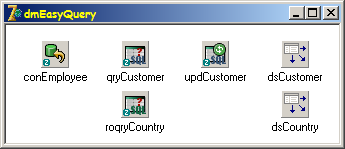
\includegraphics[width=0.7\textwidth]{ZeosTutorial/dmEasyQuery.png}
  \caption{dmEasyQuery}
  \label{fig:dmEasyQuery}
\end{figure}

TZConnection:
\begin{itemize}
  \item Database: Employee.fdb
  \item Name: conEmployee
  \item Password: "password"
  \item Protocol: firebird-1.5
  \item ReadOnly: False
  \item TransactionIsolationLevel: tiReadCommitted
  \item User: "username"
\end{itemize}

TZQuery:
\begin{itemize}
  \item Connection: conEmployee
  \item Name: qryCustomer
  \item RequestLive: True
  \item SQL: SELECT * FROM customer ORDER BY customer
  \item UpdateObject: updCustomer
\end{itemize}

Note: You have to create persistent TFields for all tablefields using the fieldeditor!

The OnAfterPost event of qryCustomer will be implemented like this:
\begin{verbatim}
procedure TdmEasyQuery.qryCustomerAfterPost(DataSet: TDataSet);
begin
  // Refresh of resultset to actualize (sort) data shown in DBGrid.
  qryCustomer.Refresh;
end;
\end{verbatim}

TZReadOnlyQuery
\begin{itemize}
  \item Connection: conEmployee
	\item Name: roqryCountry
	\item SQL: SELECT country FROM country ORDER BY 1
\end{itemize}

Note: You have to create persistent TFields for all tablefields using the fieldeditor!

TZUpdateSQL
\begin{itemize}
  \item DeleteSQL: created by UpdateSql editor
  \item InsertSQL: created by UpdateSql editor
  \item ModifySQL: created by UpdateSql editor
  \item Name: updCustomer
\end{itemize}

The delete-, insert- and modify-statements for the TZUpdateSQL object are created with the UpdateSQL editor, automatically.
The editor will be activated by double clicking on the TZUpdateSQL component.
As key field you have to select the field CUST\_NO. The fields ADDRESS\_LINE1, ADDRESS\_LINE2, CITY, STATE\_PROVINCE, COUNTRY und POSTAL\_CODE will selected as update fields in list "Update Fields".
Now the statements will be generated by clicking button "Generate SQL" (see firgures \ref{fig:dmEasyQuery_updCustomer_options} and \ref{fig:dmEasyQuery_updCustomer_sql}).
If you only have such easy queries you can save a lot of typing by using the UpdateSQL editor.
If it gets a little more complex you should create the needed statements "by hand".

\begin{figure}[htbp] 
  \centering
  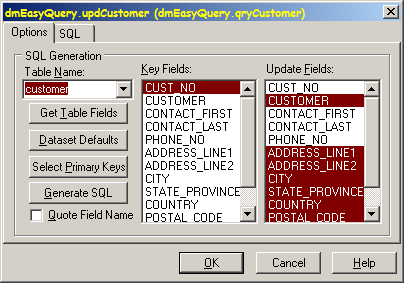
\includegraphics[width=0.7\textwidth]{ZeosTutorial/dmEasyQuery_updCustomer_options.png}
  \caption{options tab in UpdateSQL editor updCustomer}
  \label{fig:dmEasyQuery_updCustomer_options}
\end{figure}

\begin{figure}[htbp] 
  \centering
  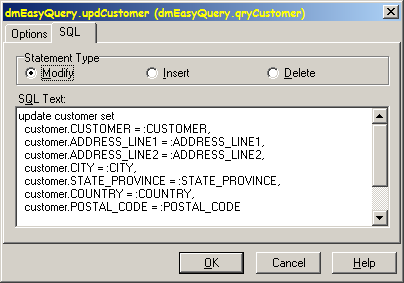
\includegraphics[width=0.7\textwidth]{ZeosTutorial/dmEasyQuery_updCustomer_sql.png}
  \caption{SQL tab in UpdateSQL editor updCustomer}
  \label{fig:dmEasyQuery_updCustomer_sql}
\end{figure}
	
TDataSource
\begin{itemize}
  \item DataSet: sqlCustomer
  \item Name: dsCustomer
\end{itemize}

TDataSource
\begin{itemize}
  \item DataSet: rosqlCountry
	\item Name: dsCountry
\end{itemize}

Now the created DataModule will be saved as dm\_EasyQuery.pas.

\section{Components for the form}
\begin{figure}[htbp] 
  \centering
  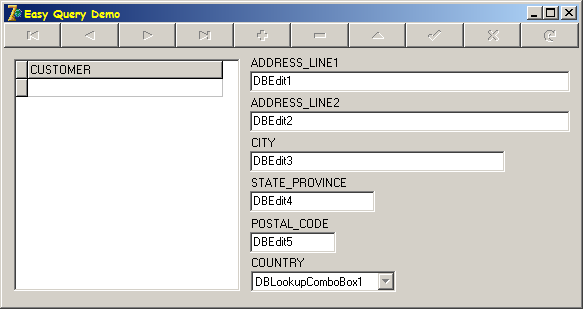
\includegraphics[width=0.7\textwidth]{ZeosTutorial/frmEasyQuery.png}
  \caption{EasyQuery main form}
  \label{fig:frmEasyQuery}
\end{figure}

The main form will have the following components and is initialized as follows:

Properties:
\begin{itemize}
  \item Caption: Easy Query Demo
  \item Name: frmEasyQuery
\end{itemize}

In the Unit's interface you have to add dm\_EasyQuery to the uses clause to get access to the database components.

The following events of the main form have to be implemented:

OnCreate:
When creating the form the connection to the database will be established.
After connecting to the database the queries will be opened:
\begin{verbatim}
procedure TForm1.FormCreate(Sender: TObject);
begin
  dmEasyQuery.conEmployee.Connect;
  dmEasyQuery.qryCustomer.Open;
  dmEasyQuery.roqryCountry.Open;
end;
\end{verbatim}

OnDestroy:
When closing the application (destroying the main form) the database connection will be cut.
All queries will be closed automatically before disconnecting.
\begin{verbatim}
procedure TForm1.FormDestroy(Sender: TObject);
begin
  dmEasyQuery.conEmployee.Disconnect;
end;
\end{verbatim}

TLabel
\begin{itemize}
  \item Caption: CUSTOMER
\end{itemize}

TDBGrid
\begin{itemize}
  \item DataSource: dmEasyQuery.dsCustomer
	\item Options.dgTabs: False
\end{itemize}

In column editor we will create a TColumn setting its property FieldName to "CUSTOMER".
After that the according column in DBGrid1 will be enlarged.

\begin{figure}[htbp] 
  \centering
  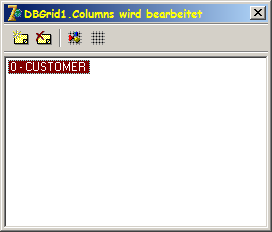
\includegraphics[width=0.7\textwidth]{ZeosTutorial/dbgrid1_columns.png}
  \caption{columns editor of DBGrid1}
  \label{fig:dbgrid1_columns}
\end{figure}

TDBEdit
\begin{itemize}
  \item (5x)
\end{itemize}

TLabel
\begin{itemize}
  \item (5x)
\end{itemize}

These objects will be created by using the columneditor of qryCustomer:
Select columns ADDRESS\_LINE1, ADDRESS\_LINE2, CITY, STATE\_PROVINCE and POSTAL\_CODE and drag and drop them onto then main form.
Align them and adapt them to the layout you see in the screenshot (figure \ref{fig:frmEasyQuery}).

TLabel
\begin{itemize}
  \item Caption: COUNTRY
\end{itemize}

TDBLookUpComboBox
\begin{itemize}
  \item DataField: COUNTRY
	\item DataSource: dmEasyQuery.dsCustomer
	\item KeyField: COUNTRY
	\item ListField: COUNTRY
	\item ListSource: dmEasyQuery.dsCountry
\end{itemize}

TDBNavigator
\begin{itemize}
  \item DataSource: dmEasyQuery.dsCustomer
\end{itemize}

Now the created form will be saved as frm\_EasyQuery.pas.

Note: The following project options have to be changed:

dmEasyQuery has to be placed on top of the creation order in list "Create automatically".
This ensures that all objects of frmEasyQuery may access the database objects.
frmEasyQuery is still the main form (see figure \ref{fig:EasyQuery_ProjectOptions}).
	
\begin{figure}[htbp] 
  \centering
  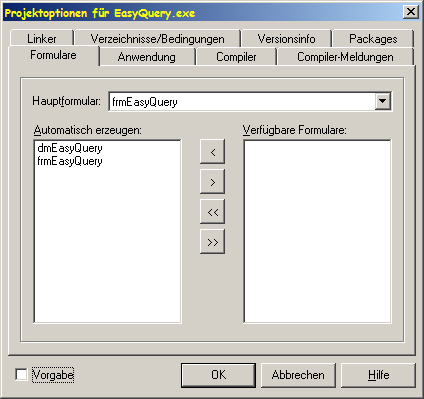
\includegraphics[width=0.7\textwidth]{ZeosTutorial/EasyQuery_ProjectOptions.png}
  \caption{EasyQuery project options}
  \label{fig:EasyQuery_ProjectOptions}
\end{figure}

\chapter{Additional Examples}
FishFact:
This is the most popular database demo for Delphi. It was migrated to use ZEOS components.

Transactions:
A sample application concerning "transactions with ZEOS". It uses a small self made test database.

StoredProc:
This is a sample applikation that shows how to use stored proecedures. The database is the Firebird
Employee sample database.

MasterDetail:
A small application that shows how master/detail connections (server and client sided) will be implemented.

EventDemo:
Also a Delphi database sample that was migrated from IBX to ZEOS.
It uses the component TIBEventAlerter.
This application needs the database Events (shipped with Delphi) that had to be migrated to dialect 3 to get this sample running.

\part{An Introduction To ZDBC API}
This document has been recovered from the original Zeoslib Foum Knoledge Base.

Zeos Database Connectivity Interface (or ZDBC for short) is a low-level API used by ZeosDBO to "hide" differences in native database client APIs and provide a uniform interface for high-level component layers. Originally, ZDBC was a port of JDBC 2.0 (Java Database Connectivity API) to Object Pascal. Since that time the API was slightly extended but the main ideas remain unchanged.

The main purpose of ZDBC is to be an intermediate layer in ZeosDBO. But it is also useful for application programming as it provides extremely light and fast access to SQL databases.

The best way to master ZDBC is to study the JDBC 2.0 specification http://java.sun.com/products/jdbc/jdbc20.pdf and then use analogy to convert JDBC abstractions and calls to ZDBC. To understand the role of ZDBC API in ZeosDBO architecture you may look at the Architecture Overview document http://www.zeoslib.net/modules.php?name=News\&file=article\&sid=23\&mode=\&order=0\&thold=0 For those who prefer a simpler introduction to ZDBC we propose a "hackers" guide as a starting point. 

\chapter{Pros and Cons of using ZDBC}
Before coding let's think why and when we should use ZDBC. Using ZDBC in applications has some clear benefits:
\begin{itemize}
  \item It's extremely fast and lightweight.
  \item It's database independent and supports many SQL servers. All supported SQL databases in ZeosDBO have correspondent ZDBC drivers.
  \item It does not require DB unit to be present. Some Personal Editions of Borland compilers do not include the DB unit with the TDataset implementation. This prevents the use of ZeosDBO components with these compilers.
\end{itemize}

There are also a few disadvantages which you need to consider carefully: 
\begin{itemize}
  \item It's not portable. You won’t be able to switch to other products without major changes in your applications (except Java and JDBC of course).
  \item It doesn't provide binding with data-aware visual controls. Implementation of such bindings manually can be a Herculean job.
  \item It doesn't contain all functionality of TDatasets such as client-side filtering, master-detail linking, sorting, etc.
\end{itemize}

So, from our point of view usage of ZDBC makes sense only in few special situations (of course you may have your personal opinion):
\begin{itemize}
  \item Your application is a console type application or does not allow users to edit relational data directly.
  \item Database access performance is very important.
  \item You don't care about porting your application to other database connectivity products.
\end{itemize}

\chapter{Establishing Connections}
In JDBC/ZDBC the entry point to the API is a special DriverManager object which serves as a factory for database connections. 

\begin{verbatim}
uses ZDbcIntfs...
...
var
  Connection: TZConnection;
...
Connection := DriverManager.GetConnection(<Connection URL>);
...
\end{verbatim}

Connection URL also comes from JDBC and has the following format:
\begin{verbatim}
zdbc:<protocol>://<host>[:<port>]/<database>[?<param1>[=<value1>]...]
\end{verbatim}

Protocol is essentially the name of the ZDBC driver you want to use. ZeosDBO version 6.1 has a number of protocols:
\begin{itemize}
  \item MySQL: mysql, mysql-3.20, mysql-3.23, mysql-4.0
	\item PostgreSQL: postgresql, postgresql-6.5, postgresql-7.2, postgresql-7.3
	\item Interbase: interbase, interbase-5, interbase-6
	\item Firebird: firebird, firebird-1.0, firebird-1.5
	\item Sybase: sybase
	\item MS SQL: mssql
	\item ADO: ado
\end{itemize}

Parameters in the connection URL specify different switches for the drivers.
There are several standard parameters for all drivers.
For other driver-specific parameters you need to refer to the ZeosDBO documentation. 
\begin{itemize}
  \item username – user name to connect to the database.
  \item password – user password to connect to the database.
  \item defaults \[yes \| no\] – calculate default values.
  \item update \[changed \| all\] – update only changed or all fields.
  \item where \[keyonly \| all\] – include where clause only key or all fields.
\end{itemize}

For example, to connect to MySQL 4.0 database with the compression protocol enabled you need to write:
\begin{verbatim}
uses ZDbcIntfs...;

...
var
  Connection: TZConnection;
...
Connection := DriverManager.GetConnection(
  'zdbc:mysql-4.0://localhost:3306/mydb?'
  + 'username=myuser;password=mypwd;compress=yes');
...
\end{verbatim}

If you want, you may specify the login and password separately: 

\begin{verbatim}
...
Connection := DriverManager.GetConnectionWithLogin(
  'zdbc:mysql-4.0://localhost:3306/mydb'
  + '?compress=yes', 'myuser', 'mypwd');
...
\end{verbatim}

Or you may specify parameters in a TStringList object:

\begin{verbatim}
...
var
  Connection: IZConnection;
  Params: TStrings;
...
Params := TStringList.Create;
Params.Values['username'] := 'myuser';
Params.Values['password'] := 'mypwd';
Params.Values['compress'] := 'yes';

Connection := DriverManager.GetConnectionWithParams(
  'zdbc:mysql-4.0://localhost:3306/mydb', Params);
\end{verbatim}

\chapter{Executing SQL statements}
We already know how to connect to our SQL database. But to do something useful you need to execute SQL statements. Let's look how to do that.

The simplest way to execute static SQL statements is the following:
\begin{verbatim}
var
  ...
  Statement: IZStatement;
  UpdatedRows: Integer;
...
Statement := Connection.CreateStatement;
UpdatedRows := Statement.ExecuteUpdate(
  'UPDATE MyTable SET MyField=''abc'' WHERE MyKey=123');
...
\end{verbatim}

Additionally to static SQL queries you can execute queries with parameters.
In some cases they may be more efficient because the parsing step is skipped.
But some SQL databases like MySQL or PostgreSQL don't support that feature and queries with parameters are emulated on the client side. 

\begin{verbatim}
var
  ...
  Statement: IZPreparedStatement;
  UpdatedRows: Integer;
...
Statement := Connection.PrepareStatement(
  'UPDATE MyTable SET MyField=? WHERE MyKey=?');

// Execute first update
Statement.SetString(1, 'abc');
Statement.SetInt(2, 123);
Statement.ExecutePrepared;

// Execute second update
Statement.SetString(1, 'xyz');
Statenent.SetInt(2, 789);
Statement.ExecutePrepared;
...
\end{verbatim}

If you execute several SQL queries one by one it makes sense to group them together in a single "batch update". 

\begin{verbatim}
...
Statement.AddBatch('UPDATE MyTable SET MyField=''abc'' WHERE MyKey=123');
Statement.AddBatch('UPDATE MyTable SET MyField=''xyz'' WHERE MyKey=789');
Statement.ExecuteBatch;
...
\end{verbatim}

Batch updates are also supported for prepared statements (statements with parameters): 

\begin{verbatim}
...
Statement := Connection.PrepareStatement(
  'UPDATE MyTable SET MyField=? WHERE MyKey=?');

// Execute first update
Statement.SetString(1, 'abc');
Statement.SetInt(2, 123);
Statement.AddBatchPrepared;

// Execute second update
Statement.SetString(1, 'xyz');
Statenent.SetInt(2, 789);
Statement.AddBatchPrepared;

Statement.ExecuteBatch;
...
\end{verbatim}

\chapter{Error Handling}
If any errors on the client or server side happens, ZDBC raises an EZSQLException exception.
This exception let you know not only the error message but also the error code from the server

\begin{verbatim}
try
  ...
  Statement.ExecuteUpdate(...);
   ...
catch
  on E: EZSQLException do
    WriteLn(Format('SQL Error: %d with Code: %d',
      [E.Message, E.ErrorCode]));
end;
\end{verbatim}

\chapter{Transaction Management}
Transaction management in ZDBC is controlled by the Connection object.
By default, Connection works in AutoCommit mode but it also provides you with all necessary methods to manage transactions manually.
Let's look how to execute SQL statements in a read-commited transaction:

\begin{verbatim}
...
Connection.SetAutoCommit(False);
Connection.SetTransactionIsolation(tiReadCommited);
...
try
  ...
  Statement.ExecuteUpdate(...);
  Statement.ExecuteUpdate(...);
  ...
  Statement.Commit;
except
  Statement.Rollback;
end;
...
\end{verbatim}

Please note that there is no out-of-transaction state.
Your connection object is always in-transaction so you don't need to start transactions manually.
Connection starts a transaction automatically when:
\begin{itemize}
  \item A connection is established
  \item AutoCommit or TransactIsolation level are changed
  \item Commit or Rollback are executed
\end{itemize}

JDBC considers this a safer approach.
You just need to be careful and complete transactions explicitly when you change AutoCommit or TransactionIsolation properties. 

\chapter{Retrieving data from SQL server}

Getting data from your SQL server may be the most interesting part of the story. Fortunately, it's not much more complicated than what we have seen so far. ZDBC API has two abstractions for queries: IZResultSet and IZResultSetMetadata. IZResultSet provides access to relational data retrieved as a result of executing a SELECT statement or a stored procedure. IZResultSetMetadata contains metadata for the query like: number of columns, column names and their types, etc.

The following example shows how to execute a SELECT statement and read its data:

\begin{verbatim}
var
...
  ResultSet: IZResultSet;
  Metadata: IZResultSetMetadata;
...
Statement := Connection.CreateStatement;
ResultSet := Statement.ExecuteQuery('SELECT * FROM MyTable');
Metadata := ResultSet.GetMetadata;

// Printing column headers
for I := 1 to Metadata.GetColumnCount do
  Write(Metadata.GetColumnName(I), ' ');
WriteLn;

// Printing query data
while ResultSet.Next do
begin
  for I := 1 to Metadata.GetColumnCount do
    Write(ResultSet.GetString(I), ' ');
  WriteLn;
end;
...
\end{verbatim}

SQL Queries can also contain parameters. Look at the next example to see how to use them:

\begin{verbatim}
...
var
...
  Statement: IZPreparedStatement;
  ResultSet: IZResultSet;
...
Statement := Connection.PrepareStatement(
  'SELECT * FROM MyTable WHERE MyKey=?');
Statement.SetInt(1, 123);
ResultSet := Statement.ExecuteQueryPrepared;
...
\end{verbatim}

The good news about ZDBC is that it allows you not only to read but also to write data.
You just need to set a ResultSetConcurrency mode for the Statement object.

\begin{verbatim}
...
Statement.SetResultSetConcurrency(rcUpdatable);
Statement.SetResultSetType(rtScrollInsensitive);
ResultSet := Statement.ExecuteQuery('SELECT * FROM MyTable');

...
// Insert a new row
ResultSet.MoveToInsertRow;
ResultSet.UpdateInt(1, 123);
ResultSet.UpdateString(2, 'abc');
ResultSet.InsertRow;
...
// Update row
ResultSet.UpdateString(2, 'xyz');
ResultSet.UpdateRow;
...
// Delete row
ResultSet.DeleteRow;
...
\end{verbatim}

\chapter{Advanced Topics}
This description of ZDBC API is not full. ZDBC has many other features like Database Metadata, Blobs, Cached Updates, Stored Procedures, Sequence Generators, etc. Unfortunately, due to size constraints, we couldn't discuss all of these topics in this article. If you want to explore more of ZDBC you need to look at the JDBC specification and the source code of the ZDbcIntfs unit for more information.

(c) 2005 ZeosLib Team

\end{document}
